\section{Porównanie wydajności}

\begin{figure}
\centering
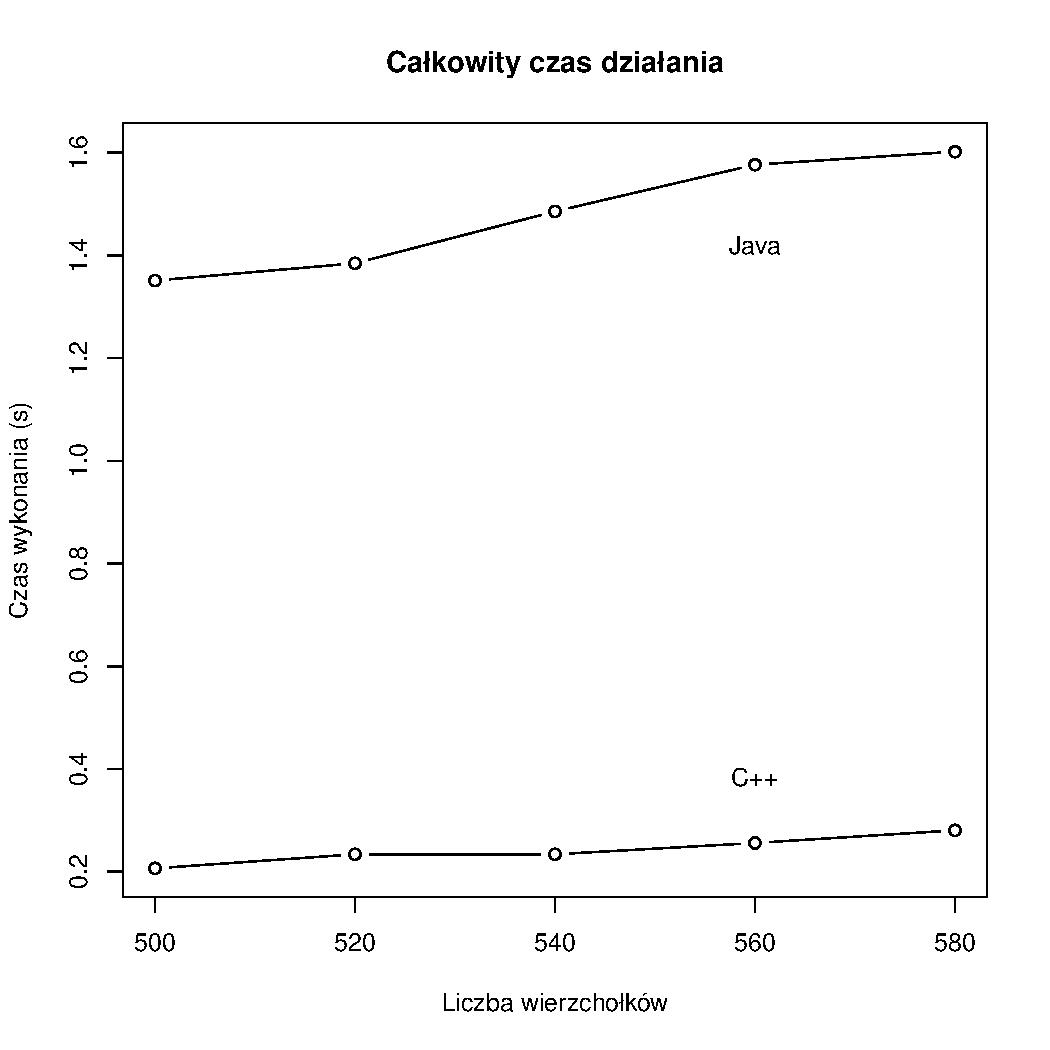
\includegraphics[scale=0.7]{plots/allTimeCompare.pdf}
\caption{Całkowity czas wykonywania zadania.}
\label{p:AllTimeCompare}
\end{figure}

\begin{figure}
\centering
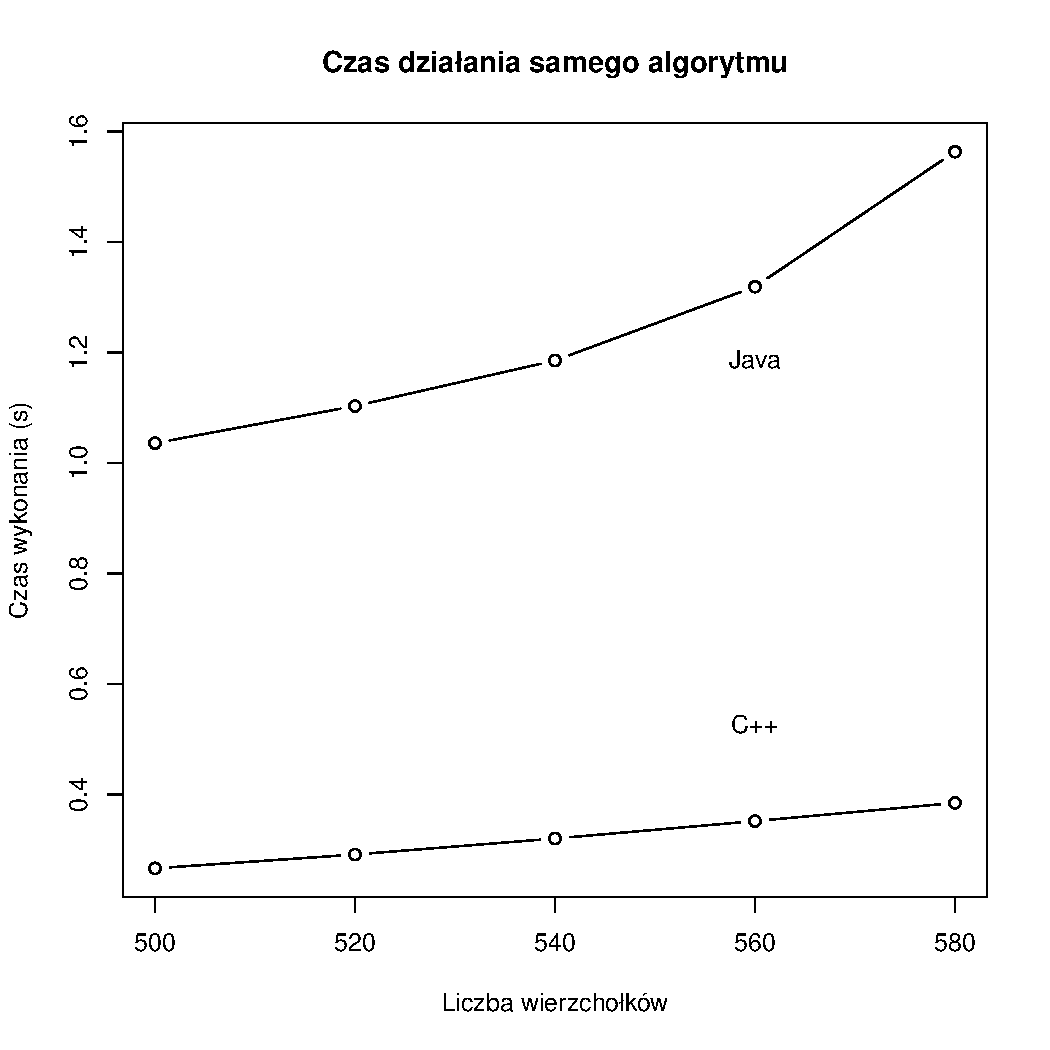
\includegraphics[scale=0.7]{plots/algTimeCompare2.pdf}
\caption{Czas działania algorytmu.}
\label{p:AlgTimeCompare}
\end{figure}

Pierwszy eksperyment reprezentuje wykres \ref{p:AllTimeCompare}.
Nie jest to zbyt sprawiedliwe porównanie, ponieważ pokazuje czas całkowitego uruchomienia (od startu do zwrócenia wyniku).
Z tego powodu, w przypadku implementacji Javy jest również uwzględniany narzut czasowy startu interpretera -- maszyny wirtualnej Javy.

Z tego powodu powstaje pytanie: Czy takie porównanie ma sens? Odpowiedź brzmi: tak, ale wyłącznie z punktu widzenia użytkownika.
Dla niego nie jest istotne w jakiej technologii jest stworzona aplikacja, lecz jak działa.
W tym przypadku widać, że aplikacja Javy zmusza do kilkukrotnie dłuższego oczekiwania na wynik.

Dla usunięcia obciążenia interpretera Javy czas został zmierzony również wewnątrz aplikacji.
Zastosowano rozdzielczość jednej mikrosekundy. 
Wynik przedstawia wykres \ref{p:AlgTimeCompare}.
Jednak jak widać, narzut ten był spory wyłącznie, dla mniejszych danych wejściowych.
Dalej odgrywał już mniejszą rolę.

\subsection{Schemat eksperymentu}

Oba eksperymenty przedstawione na wykresach \ref{p:AllTimeCompare} i \ref{p:AlgTimeCompare}
są wykonane według podobnego schematu:

\begin{enumerate}
\item Generacja (losowanie) grafów o wymaganych własnościach (np. liczbie wierzchołków, krawędzi, itp.)
\item Dla każdego grafu:
	\begin{enumerate}
		\item Kilkukrotne uruchomienie każdej implementacji -- pomiar czasu każdego uruchomienia.
		\item Średnia z powyższych pomiarów jest traktowana jako czas pracy dla określonych danych wejściowych (grafu).	
	\end{enumerate}
\item Tworzenie wykresu.
\end{enumerate}


\subsection{Złożoność}

W paragrafie \ref{sub:testy_akceptacyjne} zostało pokazane, iż aplikacje działają poprawnie.
Jednak należy również zweryfikować złożoność czasową obu rozwiązań.

\begin{figure}
\centering
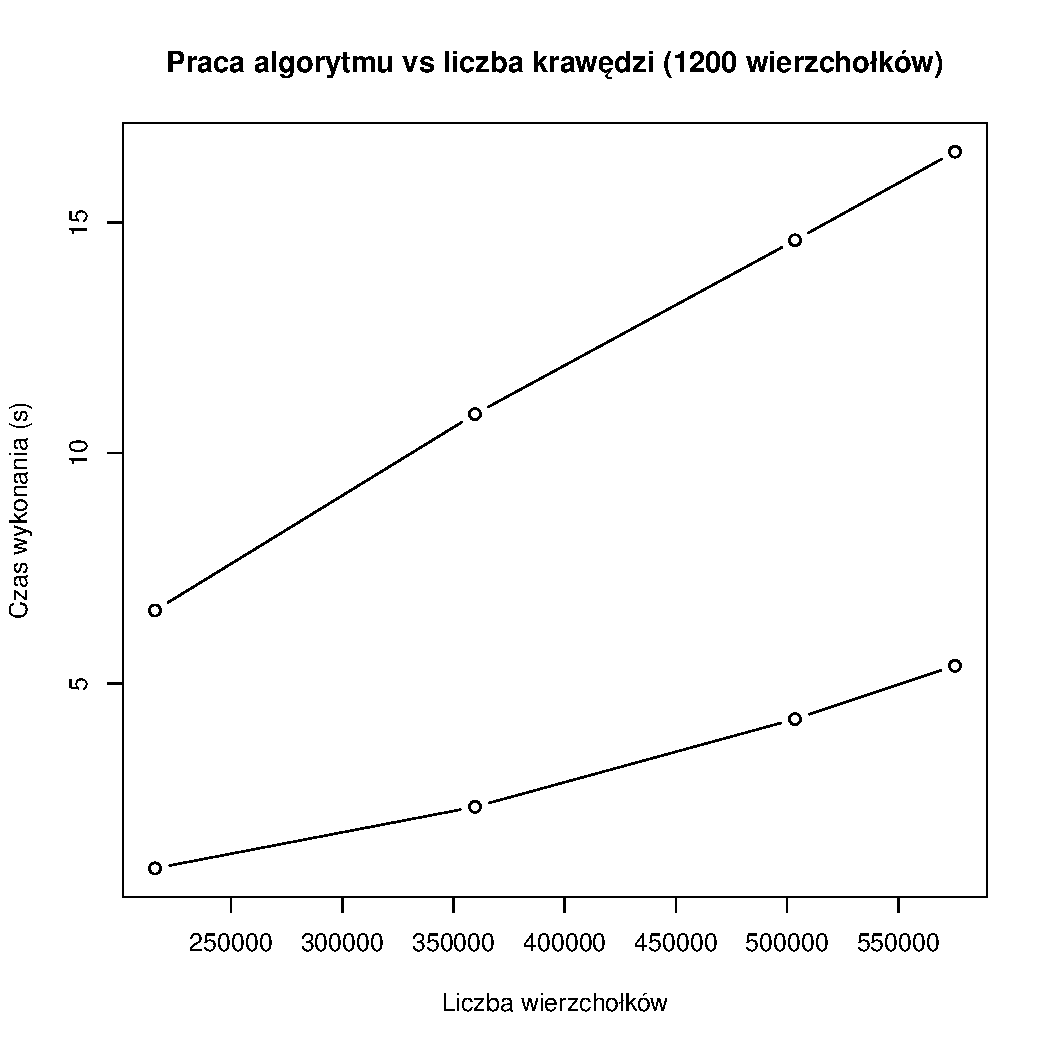
\includegraphics[scale=0.7, trim=0mm 12mm 0mm 0mm, clip]{plots/algTime_vs_edges.pdf}
\caption{Praca algorytmu w zależności do liczby krawędzi. Górny wykres -- Java, dolny -- C++.}
\label{p:AlgTime_vs_edges}
\end{figure}

Jak wskazano w poprzedniej dokumentacji, algorytm Fleury'ego ma złożoność liniową względem liczby krawędzi w grafie. 
W celu weryfikacji tego stwierdzenia, wygenerowano zbiór grafów, każdy o 1200 wierzchołkach ale różnych gęstościach.
Przeliczając gęstość na liczbę krawędzi otrzymano zbiór grafów o licznościach krawędzi pomiędzy 100 tys., a 600 tys.
Wykres \ref{p:AlgTime_vs_edges} pokazuje opisywaną tutaj zależność. 

Jednym z podstawowych wniosków jest fakt, że obie implementacje bezsprzecznie spełniają założenia algorytmu i posiadają złożoność liniową względem liczby krawędzi (O(q), gdzie $q$ to liczba krawędzi).
Ale dodatkowo można zwrócić uwagę na nachylenia obu krzywych.
Okazuje się, że zapotrzebowanie na czas rośnie szybciej w przypadku implementacji w Javie.
Nie jest to wzrost zatrważający, ale może być znaczącym argumentem do zastosowania optymalizacji w postaci zmiany języka z Javy na C++.
Szczególnie wtedy, kiedy wiadomo, że często rozpatrywane będą grafy zbliżone do pełnych.


\subsection{Rozrzut wyników}

Realizując serię pomiarów dla pojedynczej instancji problemu (w tym przypadku -- pojedynczego grafu), należy zauważyć, że każdy pomiar jest realizacją pewnej zmiennej losowej.
Przy porównywaniu obu aplikacji interesujące jest również to jak stabilne są prezentowane wyniki.

\begin{figure}
\centering
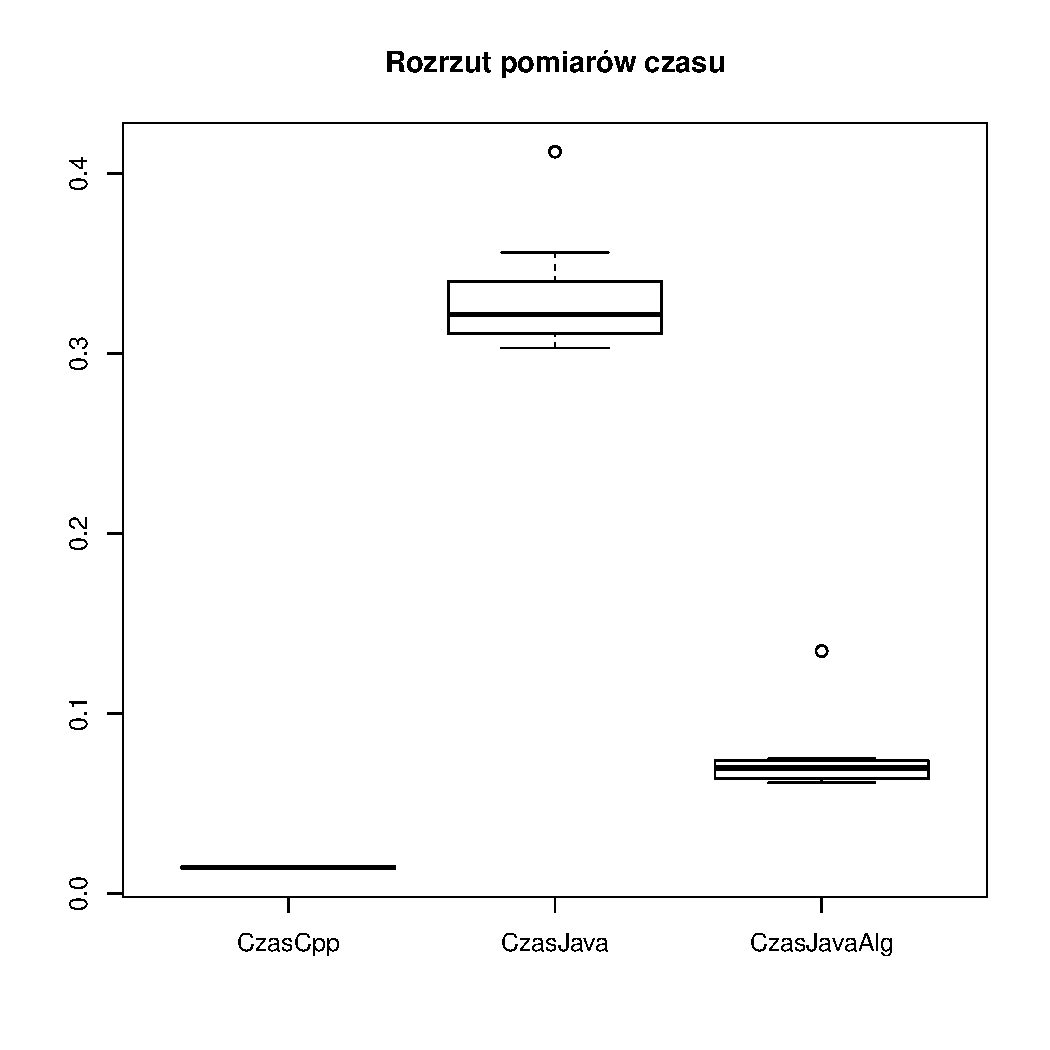
\includegraphics[scale=0.7]{plots/boxPlots.pdf}
\caption{Wykresy pudełkowe: czasu wykonania dla C++, pełnego Javy oraz samego algorytmu w Javie.}
\label{p:BoxPlot}
\end{figure}

Do interpretacji cech statystycznych wykonywanych pomiarów zastosowano wykres pudełkowy (ang. \textit{Box plot}) przedstawiony na Wykresie \ref{p:BoxPlot}.

Największy rozrzut wyników można zaobserwować w przypadku badania pełnego uruchomienia aplikacji w Javie, co może być istotne dla użytkownika końcowego.
Z drugiej strony jest to fakt w pełni uzasadniony działaniem maszyny wirtualnej Javy i systemu operacyjnego.

Dlatego do porównania lepiej zastosować pomiar pracy samego algorytmu, który w tym przypadku pokazuje stabilniejsze działanie. 
Jednak również w tej kategorii niepokonana została implementacja z wykorzystaniem C++. 
Dla której wahania były tak niewielkie, że z racji skali wykresu \ref{p:BoxPlot}, są one niewidoczne.


\subsection{Serie uruchomień}

Na koniec warto przyjrzeć się jeszcze zmienności wyników w perspektywie serii uruchomień każdej z implementacji -- rysunki \ref{p:cppSeries} oraz \ref{p:javaSeries}.

Pokazują one cechę odporności obu implementacji na zmienną gęstość tych samych grafów.
Wyniki są zgodne z oczekiwaniami -- uzyskano zależność liniową -- ale nie jest to cecha oczywista i automatyczna. 
Gdyby w którymś rozwiązaniu zastosowano niewłaściwą strukturę danych (a co za tym idzie nieefektywną), można by zaobserwować znaczące fluktuacje na poszczególnych krzywych.

\begin{figure}
\centering
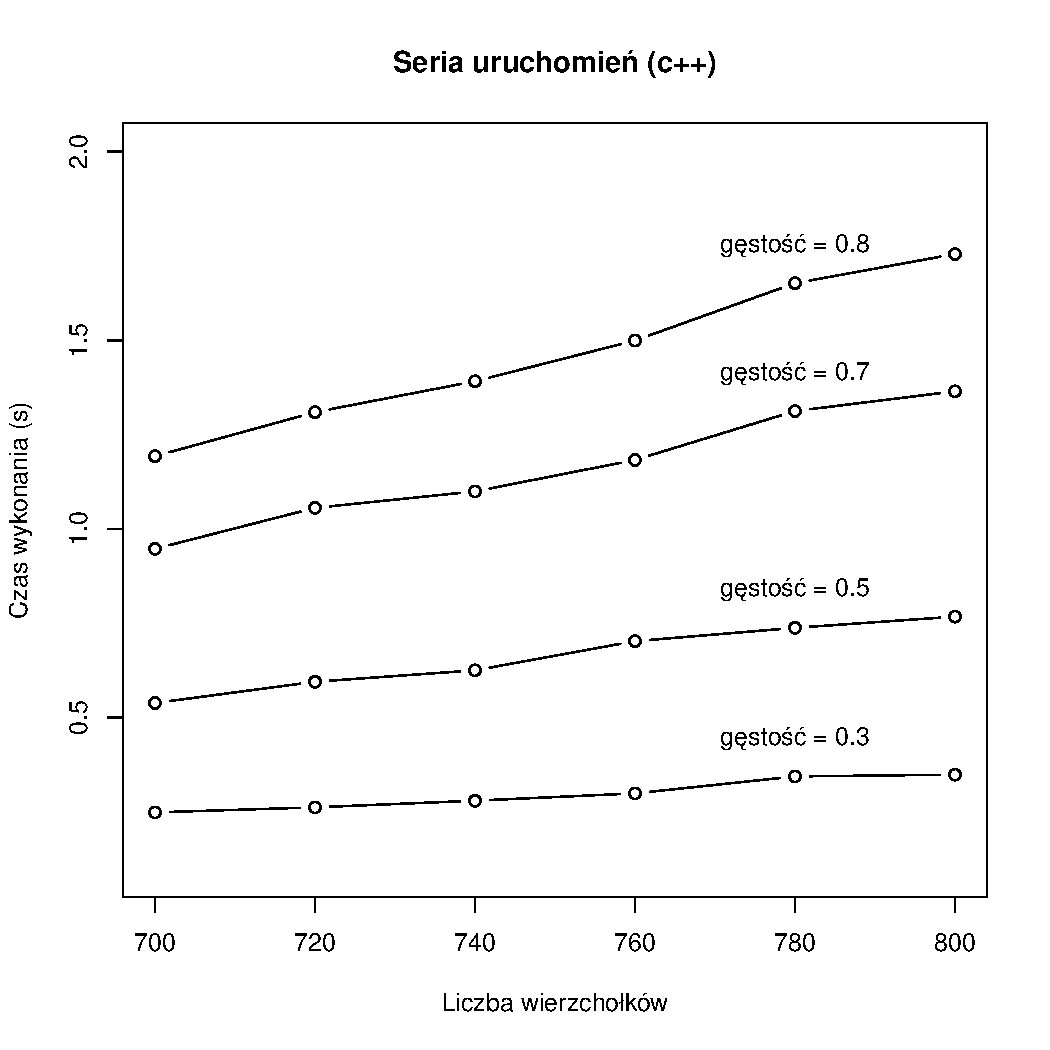
\includegraphics[scale=0.6]{plots/cppTime_inSeries.pdf}
\caption{Seria uruchomień aplikacji napisanej w C++.}
\label{p:cppSeries}
\end{figure}

\begin{figure}
\centering
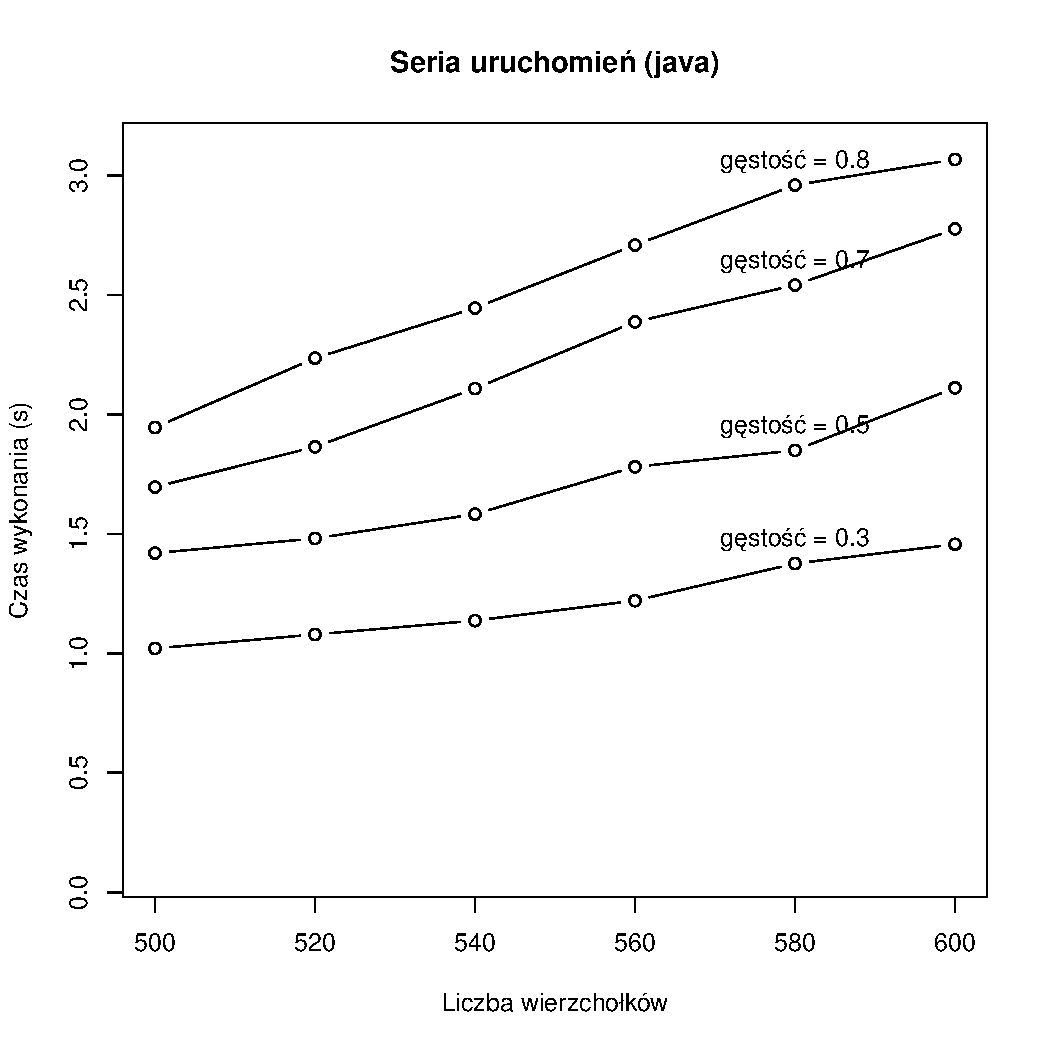
\includegraphics[scale=0.6]{plots/javaTime_inSeries.pdf}
\caption{Seria uruchomień aplikacji napisanej w Javie.}
\label{p:javaSeries}
\end{figure}